% 
% This message contains the LaTeX template for scribe notes
% in EE597.  You are free to use other means of producing
% your notes, but you are encouraged to use LaTeX: you will
% need to learn it some day.
% 
% Many thanks to Alistair Sinclair@cs.berkeley.edu for providing the basis for
% the first version of this template.
% 
% %************************************************************
%
% This is the LaTeX template file for lecture notes for EE596
% Pattern Recognition II: Introduction to Graphical Models.  When preparing 
% LaTeX notes for this class you must use this template.
%
% To familiarize yourself with this template, the body contains
% some examples of its use.  Look them over.  Then you can
% run LaTeX on this file.  After you have LaTeXed this file then
% you can look over the result either by printing it out with
% dvips or using xdvi.
%

\documentclass{article}
\usepackage{times,amsmath,amsthm,amsfonts,eucal,graphicx,algorithm,algpseudocode}


% This scribe template not only uses latex, but also
% the American Mathematical Society (AMS) latex macros.
% Detailed documentation on how to use them to produce good
% math formating can be obtained here: http://www.ams.org/tex/
% I've also placed a copy of the AMS-Latex documentation
% on the web page at:
%     http://www.ee.washington.edu/class/596/patrec/scribes/amsguide_2p.ps
% Latex documentation can be obtained from 
%
% Publications related to latex are listed here:
%     http://www.ams.org/tex/publications.html
%

\setlength{\oddsidemargin}{0.25 in}
\setlength{\evensidemargin}{-0.25 in}
\setlength{\topmargin}{-0.6 in}
\setlength{\textwidth}{6.5 in}
\setlength{\textheight}{8.5 in}
\setlength{\headsep}{0.75 in}
\setlength{\parindent}{0 in}
\setlength{\parskip}{0.1 in}

%
% The following commands set up the lecnum (lecture number)
% counter and make various numbering schemes work relative
% to the lecture number.
%
\newcounter{lecnum}
\renewcommand{\thepage}{\arabic{page}}
\renewcommand{\thesection}{\arabic{section}}
\renewcommand{\theequation}{\arabic{equation}}
\renewcommand{\thefigure}{\arabic{figure}}
\renewcommand{\thetable}{\arabic{table}}

%
% A few symbols that we will be using often in this course.
\newcommand{\indep}{{\bot\negthickspace\negthickspace\bot}}
\newcommand{\notindep}{{\not\negthickspace\negthinspace{\bot\negthickspace\negthickspace\bot}}}
\newcommand{\definedtobe}{\stackrel{\Delta}{=}}
\renewcommand{\choose}[2]{{{#1}\atopwithdelims(){#2}}}
\newcommand{\argmax}[1]{{\hbox{$\underset{#1}{\mbox{argmax}}\;$}}}
\newcommand{\argmin}[1]{{\hbox{$\underset{#1}{\mbox{argmin}}\;$}}}

%
% The following macro is used to generate the header.
%
\newcommand{\lecture}[4]{
   \pagestyle{myheadings}
   \thispagestyle{plain}
   \newpage
   \setcounter{lecnum}{#1}
   \setcounter{page}{1}
   \noindent
   \begin{center}
   \framebox{
      \vbox{\vspace{2mm}
    \hbox to 6.58in { {\bf [CS502]-Graph Theory and Applications
                        \hfill Fall 2021-22} }
    \hbox to 6.58in { {\bf 
                        \hfill } }
       \vspace{4mm}
       \hbox to 6.28in { {\Large \hfill A* Search Algorithm \hfill} }
       \vspace{5mm}
       \hbox to 2.28in { { \textit{Instructor: Vinod Reddy}    \hspace{7cm}  \textit{Authors: Swapnil Narad, Ambar Mutha}} }
  
}
   }
   \end{center}
   \markboth{A* Search Algorithm}{A* Search Algorithm}
   \vspace*{4mm}
}

%
% Convention for citations is authors' initials followed by the year.
% For example, to cite a paper by Leighton and Maggs you would type
% \cite{LM89}, and to cite a paper by Strassen you would type \cite{S69}.
% (To avoid bibliography problems, for now we redefine the \cite command.)
% Also commands that create a suitable format for the reference list.
\renewcommand{\cite}[1]{[#1]}
\def\beginrefs{\begin{list}%
        {[\arabic{equation}]}{\usecounter{equation}
         \setlength{\leftmargin}{2.0truecm}\setlength{\labelsep}{0.4truecm}%
         \setlength{\labelwidth}{1.6truecm}}}
\def\endrefs{\end{list}}
\def\bibentry#1{\item[\hbox{[#1]}]}

%Use this command for a figure; it puts a figure in wherever you want it.
%usage: \fig{NUMBER}{CAPTION}{.eps FILE TO INCLUDE}{WIDTH-IN-INCHES}
\newcommand{\fig}[4]{
			\begin{center}
	                \includegraphics[width=#4,clip=true]{#3} \\
			Figure \thelecnum.#1:~#2
			\end{center}
	}

\theoremstyle{definition}
% Use these for theorems, lemmas, proofs, etc.
\newtheorem{theorem}{Theorem}[lecnum]
\newtheorem{lemma}[theorem]{Lemma}
\newtheorem{proposition}[theorem]{Proposition}
\newtheorem{claim}[theorem]{Claim}
\newtheorem{corollary}[theorem]{Corollary}
\newtheorem{definition}[theorem]{Definition}
\newtheorem{problem}{Solution of problem}

% \newenvironment{proof}{{\bf Proof:}}{\hfill\rule{2mm}{2mm}}

% **** IF YOU WANT TO DEFINE ADDITIONAL MACROS FOR YOURSELF, PUT THEM HERE:

\begin{document}
%FILL IN THE RIGHT INFO.
%\lecture{**LECTURE-NUMBER**}{**DATE**}{**LECTURER**}{**SCRIBE**}
\lecture{1}{}{xxx}
%\footnotetext{These notes are partially based on those of Nigel Mansell.}

% **** YOUR NOTES GO HERE:
\section{Introduction}
Search algorithms or be more specifically pathfinding algorithms are very useful in many real-time settings like in the areas of networking, video games, robotics etc. It is used to find the shortest route between two points. Pathfinding is closely related to the shortest path problem, within graph theory. These algorithms extend from well-known graph traversals like Breadth-First Search and Depth First Search, Dijkstra’s Algorithm and Bellman’s Ford Algorithm. A* (A Star) Search Algorithm is also one of these paths finding algorithms.

For a greater understanding, we can say that Dijkstra’s Algorithm is a special case for the A* search algorithm where we take the heuristic value for each vertex as 0. In contrast to Dijkstra and others, in the A* algorithm, a heuristic approach is implemented into a standard graph search algorithm that effectively plans ahead to make the right decision. Due to its heuristic components and thus goal-oriented nature, it also has its significance in Artificial Intelligence studies. Unlike Dijkstra, A* helps us to find the shortest distance only between the starting point and the ending point.

\section{Working of the algorithm}
\subsection{Working}

In a graph with weighted edges, the A* search algorithm finds the shortest path between a source vertex S and a target vertex T or determine whether no path exists connecting S and T. It is used in a huge graph where any blind search algorithm like BFS will be very inefficient and would not be terminated in a feasible time. The algorithm tracks the vertices to check in the open set and the checked vertices in the closed set. The open set is initialized with the start vertex S and the closed set is empty.

Each vertex $v$ has a value $f(v)$ associated to it such that
\[ f(v) = g(v) + h(v) \]

where $g(v)$ is the cost required to reach the vertex $v$ from S and $h(v)$ is a heuristic value which denotes the estimated cost to reach target vertex T from $v$. For the algorithm to work correctly, the heuristic $h(v)$ can be underestimated but cannot be overestimated i.e. it should never be higher than the actual cost.

The algorithm iterates over vertices in the open set until it is empty. In each iteration, the vertex with the smallest $f(v)$ is chosen and moved from open set to closed set and its unvisited neighbors are added to the open set. If we reach the target vertex, we have found the shortest path. If the open set becomes empty without reaching the target then the source and target are not connected.

\subsection{Pseudocode}

\begin{algorithm}[H]
	\caption{Compute sum of integers in array}
	\label{array-sum}
	\begin{algorithmic}[1]
		\Procedure{A* Search}{Node S,Node T, Graph $G$}
		\State S.f $\leftarrow 0$
		\State openSet $\leftarrow \{S\}$
		\State closedSet $\leftarrow \{\}$
		\While { openSet.size $> 0$ }
		\State current $\leftarrow$ node from openSet having smallest f value
		\State openSet.remove(q)
		\If {current $==$ T}
		\State \Return path from S to T
		\EndIf
% 		\State successors $\leftarrow$ q's successors
		\For {each neighbor in current.neighbors}
		\If{neighbor in closedSet}
		\State continue
		\EndIf
		\State new\_g = current.g + cost of edge between current and neighbor
		
		\If{neighbor not in openSet}
		    \State openSet.add(neighbor)
	    \Else \If{new\_g $\geq$ neighbor.g}
	        \State continue
	        \EndIf
	    \EndIf
		\State neighbor.g = new\_g
		\State neighbor.f = neighbor.g + Estimated cost of travelling from neighbor to T
		\State neighbor.parent = current
		\EndFor
		\EndWhile
		\State \Return Error: Path does not exist
		\EndProcedure
	\end{algorithmic}
\end{algorithm}
\newpage
\subsection{Example}
We are taking an example of a undirected graph G to do a dry run for the algorithm.

\begin{center}
    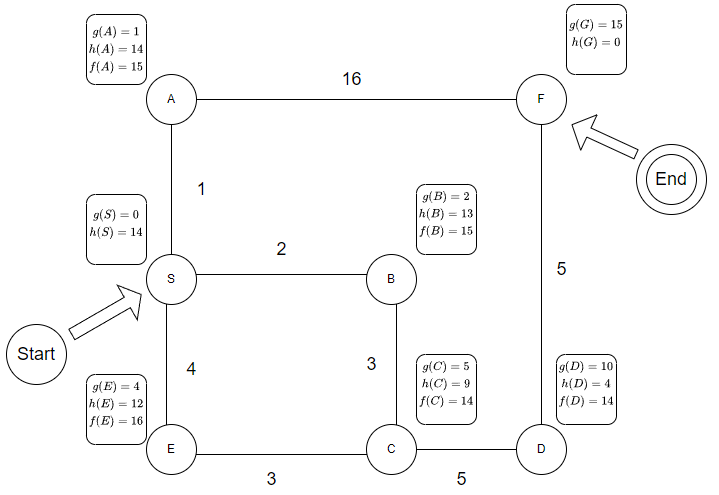
\includegraphics[width=\linewidth]{DryRun-3.png}
\end{center}
\begin{enumerate}
    \item We will start with vertex $S$ by initializing the algorithm with $g(S) = 0$ and $h(S) = 14$.
    \item We will now add neighbours of vertex $S$.
    \begin{enumerate}
        \item We will first add $A$ to open list with $g(A) = 1$, $h(A) = 14$ and $f(A) = 15$. \item Then add $B$ to open list with $g(B) = 2$, $h(B) = 13$ and $f(B) = 15$.
        \item Finally add $E$ to open list with $g(E) = 4$, $h(E) = 12$ and $f(E) = 16$.
    \end{enumerate}
    \item Here we have $f(B)$ and $f(A)$ both having least and equal value $f(A) = f(B) = 15$, so we will be adding neighbours of $A$ to open list as it entered the open list first, and therefore we will be adding $F$(which is also the end vertex) to the open list with $g(F) = 17$, $h(C) = 0$ and $f(C) = 17$. Since this is not the least value in open list, the algorithm will not stop here.
    \item Now we have the least value of $f(B) = 15$ so now we will add neighbours of $B$ to the open list, and therefore $C$ will be added with $g(C) = 5$, $h(C) = 9$ and $f(C) = 14$.
    \item Right now the least item on the open list is $f(C) = 14$, so we will be adding neighbours of it i.e. $D$ with $g(D) = 10$, $h(D) = 4$ and $f(D) = 14$.
    \item The least item in the open list is now $f(D)$, so we will add $F$ to the open list with $g(F) = 15$, $h(F) = 0$ and $f(F) = 15$, which is also the least value in the open list, since $F$ is also the end vertex or goal state and it is also having the least $f$ value in the open list, the algorithm will be terminated and we will get the path as $S \longrightarrow B \longrightarrow C \longrightarrow D \longrightarrow F$ with total cost 15.
\end{enumerate}
\subsection{Complexity Analysis}
	
	\textbf{Time Complexity}: Consider a graph that starts as a straight line path with the starting vertex on one end and the ending vertex on the other, for example -- $0$ (source) $\rightarrow 1 \rightarrow 2 \rightarrow3$(target). So the worst case time complexity is $\mathcal{O}(E)$, where E is the number of edges in the graph.
	
	\textbf{Auxiliary Space}: In the worst case we can have all the edges inside the open list, so required auxiliary space in the worst case is $\mathcal{O}(V)$, where $V$ is the total number of vertices.
	
	\subsection{Heuristic Functions}
	The choice of Heuristic Function is the most important part of determining the efficiency of the A* search algorithm. We can calculate $g(v)$ as it is definite, but as $h(v)$ is a guess, choosing the appropriate formula for determining the heuristic value should be done carefully.
	There are two ways to do so:
	
	\begin{enumerate}
		\item Calculate the exact value of $h(v)$: This will result in worst time and space complexities, this can be done in two ways:
		\begin{enumerate}
			\item We can compute the distances between every pair of nodes in advance(Pre-computation). This will be highly inefficient and infeasible with respect to space complexity $\mathcal{O}(V^2)$ that this method might demand.
			\item If no obstacle is present in the graph, then we can easily calculate the distance between two nodes by the euclidean formula.
		\end{enumerate}
		\item The other way of doing this will be by approximating the value of $h(v)$ using some heuristic formula: Based on the implementation, there can be various ways to approximate the value of $h(v)$. Some of these methods are:
		Consider $C$ $\longrightarrow$ Current Vertex and $T$ $\longrightarrow$ Target Vertex;
		\begin{enumerate}
			\item \underline{\textbf{Manhattan Distance}}: This is defined as the sum of the absolute difference between the value of $x$ coordinate of the current cell and the value of $x$ coordinate of the target cell, with the absolute difference between the value of $y$ coordinate of the current cell and the value of $y$ coordinate of the target cell, i.e,
			$$ h = | \ C.x - T.x \ | + | \ C.y - T.y \ | $$
		    We can only consider movement in four directions i.e. (up, down, left, right) while using this formula. 
			
			\item \underline{\textbf{Diagonal Distance}}: This is defined as the maximum of absolute values of differences in the target’s $x$ and $y$ coordinates and the current cell’s $x$ and $y$ coordinates respectively, i.e.,
			$$ = max(| \ C.x - T.x \ |,| \ C.y - T.y \ |) $$
			This formula can be used when we can explore in all the eight directions.
			
			\item \underline{\textbf{Euclidean Distance}}: This is the square root of the sum of the squares of the difference of x,y values of the current cell and that of the target cell, respectively., i.e,
			$$h = \sqrt{(C.x - T.x)^2 +(C.y - T.y)^2}$$
			This formula can be used when we are free to go in any directions.
		\end{enumerate}
	\end{enumerate}
\subsection{Estimation}
As we are guessing the value for our heuristic function $h(v)$, there are two cases possible other than guessing the correct distance between two points, these are:
\subsubsection{Over-Estimation}
If the guess value is more than the actual value of the distance between the current node $v$ and the target node $t$, i.e., $h(v) > d(v \rightarrow t)$,  then the approximation is termed to be overestimated. If over-estimation is made while calculating the value of $h(v)$, then the algorithm may not return the optimum distance between the starting node and the target node. This can be explained with the example given below :
\begin{center}
    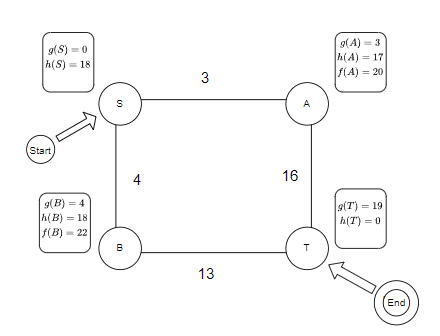
\includegraphics[scale = 0.9]{Over-Estimation.png}
\end{center}
\begin{enumerate}
    \item The open list will be initialised with the vertex $S$ with $g(S)=0$, $h(S)=18$.
    \item Now neighbours of S will be added to open list, $A$ will be inserted with $g(A) = 3$, $h(A) = 17$ and $f(A) = 20$ and $B$ will also be inserted with $g(B) = 4$, $h(B) = 18$ and $f(A) = 22$. 
    \item Since $f(A) < f(B)$, so neighbours of $A$ will be taken and therefore $T$ will be added to open list, with $g(T) = 19$, $h(t) = 0$ and $f(T) = 19$.
    \item Since $f(T)$ has the least value in open list and also $T$ is the target node and therefore the algorithm will be terminated here with path as $S \longrightarrow A \longrightarrow  T$ with total cost as 19.
    \item The optimal value of $d(S \longrightarrow T) = 17$, but the algorithm returns
19 this happened because of over-estimation in the heuristic function.
\end{enumerate}
\newpage
\subsubsection{Under-Estimation}
If the guess value is less than the actual value of the distance between the current node v and the target node $t$, i.e., $h(v) < d(v \rightarrow t)$, then the approximation is termed to be underestimated. Under-estimation guarantees the algorithm will return the optimum value, but more the underestimation, more tedious is the algorithm. This can be explained with the example given below :
\begin{center}
    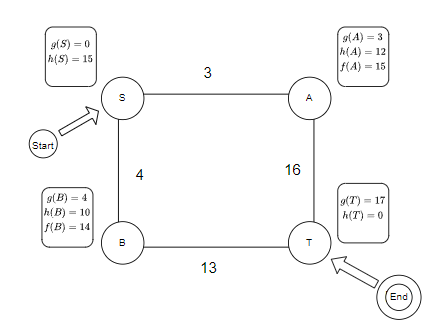
\includegraphics[scale = 0.9]{Under-Estimation.png}
\end{center}
\begin{enumerate}
    \item The open list will be initialised with the vertex $S$ with $g(S)=0$, $h(S)=15$.
    \item Now neighbours of $S$ will be added to open list, $A$ will be inserted with $g(A) = 3$, $h(A) = 12$ and $f(A) = 15$ and $B$ will also be inserted with $g(B) = 4$, $h(B) = 10$ and $f(A) = 14$. 
    \item Since $f(A) > f(B)$, so neighbours of $B$ will be taken and therefore $T$ will be added to open list, with $g(T) = 17$, $h(t) = 0$ and $f(T) = 17$.
    \item Since $f(T)$ has the least value in open list and also $T$ is the target node and therefore the algorithm will be terminated here with path as $S \longrightarrow B \longrightarrow  T$ with total cost as 17.
    \item The optimal value of $d(S \longrightarrow T) = 17$ which is also returned by the algorithm by using under-estimation.
\end{enumerate}
\section{Applications}
Path finding have a very wide range of applications, there are several industries which use path finding to a great extent, some of the fields are Networking, Game development, Robotics, AI etc.
 Computer games like CS:GO, Age Of Empires, GTA series uses path finding extensively to design their bot movement, the game's bots or in some cases AI pedestrians design their route using A* search algorithm and its variants. Cui, Xiao \& Shi, Hao [1] has already reviewed the various A* based gaming algorithms and addressed their uses in some of the popular games mentioned above in their paper. [2] and [3] have proposed robot path finding algorithms using A* algorithms. 
\subsection{Finding shortest route in a city}

A common scenario where A* Search Algorithm can be used effectively is finding route between two points in a dense city with a large number of roads and intersections.

The problem can be modeled as a graph where road intersections are represented by vertices. The start and end points are vertices S and T respectively. The roads are represented by edges connecting these vertices. The weight of each edge is the length of the road in between. And the heuristic $h(v)$ for each vertex can be defined as the euclidean distance between $v$ and T. Since the shortest route to T will always be at least as much as the euclidean distance, we are confident that our heuristic can never be an overestimate. Therefore, the A* search algorithm will always give the shortest path.

Similarly, the A* search algorithm can be used in any geographical path finding scenario.

\section{Conclusions}

To conclude, A* search algorithm is currently the best path searching algorithm and heavily optimises path searching in a large graph with obstacles between the start and target nodes. As a result, it has many real-world applications such as in navigating maps, video games and more. This algorithm's efficiency is due to the heuristic that determines which node next may provide the optimal path while ignoring any other irrelevant nodes.

\section{References}
\begin{enumerate}
    \item \textit{Cui2011AbasedPI} - A*-based Pathfinding in Modern Computer Games - Xiao Cui and H. Shi.
    \item \textit{Guruji2016} - Time-efficient A* Algorithm for Robot Path Planning - Akshay Kumar Guruji and Himansh Agarwal and D.K. Parsediya.
    \item \textit{Peng2015} - Robot Path Planning Based on Improved A* Algorithm - Jiansheng Peng and Yiyong Huang and Guan Luo.
    \item \textit{Wikipedia - Pathfinding} 
    \item \textit{Wikipedia - A*-search-algorithm}
    \item \textit{GeeksForGeeks - A*-search-algorithm}
\end{enumerate}
% Some general latex examples and examples making use of the
% macros follow.  
%**** IN GENERAL, BE BRIEF AND COMPLETE. 

% **** THIS ENDS THE EXAMPLES. DON'T DELETE THE FOLLOWING LINE:

\end{document}


